% Possible background additions:
% Positive/Negative examples ILASP.
% Semantic parsing maybe.

% Add a box plot somewhere


% TODO: Alessandra feedback: use running examples because it's easier to understand that way
\chapter{Solving NLP Tasks Logically}
\label{solving-nlp-tasks-logically}


Logical representations have an important place in the Natural Language Processing field.
Semantic parsing \cite{RefWorks:RefID:28-jurafsky2014speech} is a famous task that aims to convert a natural language input that captures the meaning of that input.
After all, having a sentence in a logical form allows reasoning about it to form new conclusions.

However, in this chapter, the logic is used in a slightly unconventional manner for NLP.
It is an intermediate representation for a sequence-to-sequence problem where it captures only the syntax of the text rather than its meaning.
The current state-of-the-art approaches for sequence-to-sequence problems, such as language translation, all use transformers. 
Nevertheless, seq2seq transformers would perform poorly with available datasets for the two problems tackled in this chapter.
The datasets consisting of ~100 examples are too small for a model with billions of parameters to be able to generalise.
% INSERT Imdb dataset reference 
Transformer fine-tuning is usually done on tens of thousands of examples, such as the IMDB Movie Reviews dataset. \\
% INSERT reference second year notes.
On the other hand, logic-based learning systems can generalise well from few examples, making them suitable for the problems presented in this chapter. 

In this chapter, we demonstrate how to solve two seq2seq NLP tasks using logical approaches, which constitute a crucial part of our concept bottleneck model (Chapter \ref{concept-bottleneck-pipeline}).
They are combined into a sentence-to-sentence transformer (note the difference between the standard transformer), shown diagrammatically in the figure \ref{sentence2sentence-transformer}.

\begin{figure}[h]
\caption{Diagrammatic representation of the sentenece2sentence transformer}
\vspace{10pt}
\centering
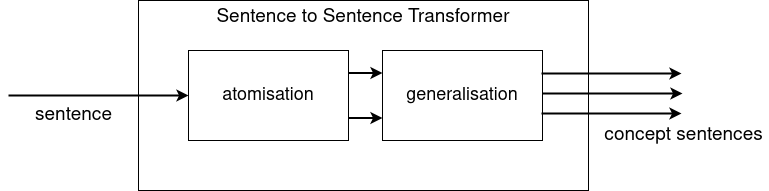
\includegraphics[width=\textwidth]{solving-nlp-tasks-logically/sent2sent_transformer.png}
\label{sentence2sentence-transformer}
\end{figure}



% TODO: Alessandra feedback: add more introduction, namely the drawing in alessandra-feedback-diagram - one box is for the atomiser (symbolic atomisation transformer), another one for generalisation - they work on sentences to sentences
% TODO: Alessandra feedback: go into how both atomisation and generalisation works briefly
% TODO: Alessandra feedback: add more introduction, namely the drawing in alessandra-feedback-diagram

% From what I understood Ale's feedback is decided on the Nuri's paper - if there is time look into his papers for inspiration
 
\section{Sequence2Sequence Tasks}
\label{sentence-type-definitions}

The two tasks that have been tackled using logic based learning approach are \textbf{sentence} \textbf{atomisation} and \textbf{generalisation}.

The former converts a declarative sentence into one or more \textbf{atomic sentences}, while the latter converts an \textbf{atomic sentence} into one or more \textbf{concept sentences}.

\textbf{Atomic Sentence:} A sentence that cannot be decomposed into multiple valid sentences. \\
% TODO add reference %
Note that this is equivalent to the definition used in logic.
However, the sentence structure considered in this project is often much more complex than the one considered in logic.\\
% INSERT insert simple predicates definition reference NOREF %
An \textbf{atomic sentence} should only contain simple predicates, eliminating compound and complete predicates from a sentence.


\textbf{Concept Sentence:} A syntactic generalisation of an atomic sentence, which satisfies the following three conditions:
\begin{enumerate}
% TODO: Alessandra feedback: valid -> syntactically well-formed -> give examples for what it means for a sentence to be syntactically well-formed
    \item It is a valid sentence in its own right.
    \item True if the atomic sentence is.
    \item Obtained only through syntactic manipulation of an atomic sentence, a result of modifying the syntax tree of the sentence.
\end{enumerate}

% TODO: Alessandra feedback: argue that concept sentence is any syntactically well formed substring of an atomic sentence.
Concept sentences are sometimes referred to as \textbf{(syntactic) generalisations} of a sentence in this report.


\begin{example}
Splitting a given sentence into all its concepts sentences.

Starting from the sentence:  
\begin{verbatim}
The batter caught the ball in the air and sent it into the left field.
\end{verbatim}
we can extract the following atomic sentences: 
\begin{verbatim}
The batter made contact with the ball in the air. 
The batter sent it into the left field.
\end{verbatim}
From these two sentences, we can obtain four concept sentences: 
\begin{verbatim}
The batter made contact with the ball in the air.
The batter made contact with the ball.
The batter sent it into the left field.
The batter sent it into the field.
The batter sent it.
\end{verbatim}

\end{example}

These two tasks (i.e. the sentence-to-sentence transformer) serve as a replacement for the extraction part of the original CoDEx (Concept Discovery and Extraction) pipeline (\ref{inherited-work}).

Notice that both tasks are purely syntactic; one requires no understanding of the sentence to atomise/generalise it.
The benefit of a syntactic approach is its domain independence, allowing it to be seamlessly applied to sentences with a completely different meaning.
In addition, the reason the project aims to extract all concept sentences from a particular sentence is two-fold:
\begin{enumerate}
    \item Concept sentences help associate differently worded explanations of the same concept.
    \item The final generated sentences are immediately usable for explanations.
\end{enumerate}

% TODO: Alessandra feedback: argue that atomistaion is a 3-step process - generate logical form + apply rules + reconstruct the data
% TODO: Alessandra feedback: add diagram with dependency trees - alessandra feedback-diagrams.png has a sketch

% TODO: Alessandra feedback: add part 1 of the diagram from the introduction but now show the syntactic parse trees to showcase what we are doing in this part
% TODO: Alessandra feedback: argue why the atomisation task is harder than the generalisation
\section{Solving Atomisation Task}
\label{solving-atomisation-task}

The atomisation task is the more challenging of the two.
The reason is the diversity of the input the model must handle, both with respect to size and the types of tokens encountered.
The atomiser should ideally be able to process any declarative sentence, whereas the generaliser expects an atomic sentence as input, which is significantly easier to handle. 

To tackle this task, we have constructed a hand-crafted solution whose application is shown in \ref{atomisation-diagram}.

\begin{figure}[h]
\caption{Diagrammatic representation of the atomiser}
\vspace{5pt}
\centering
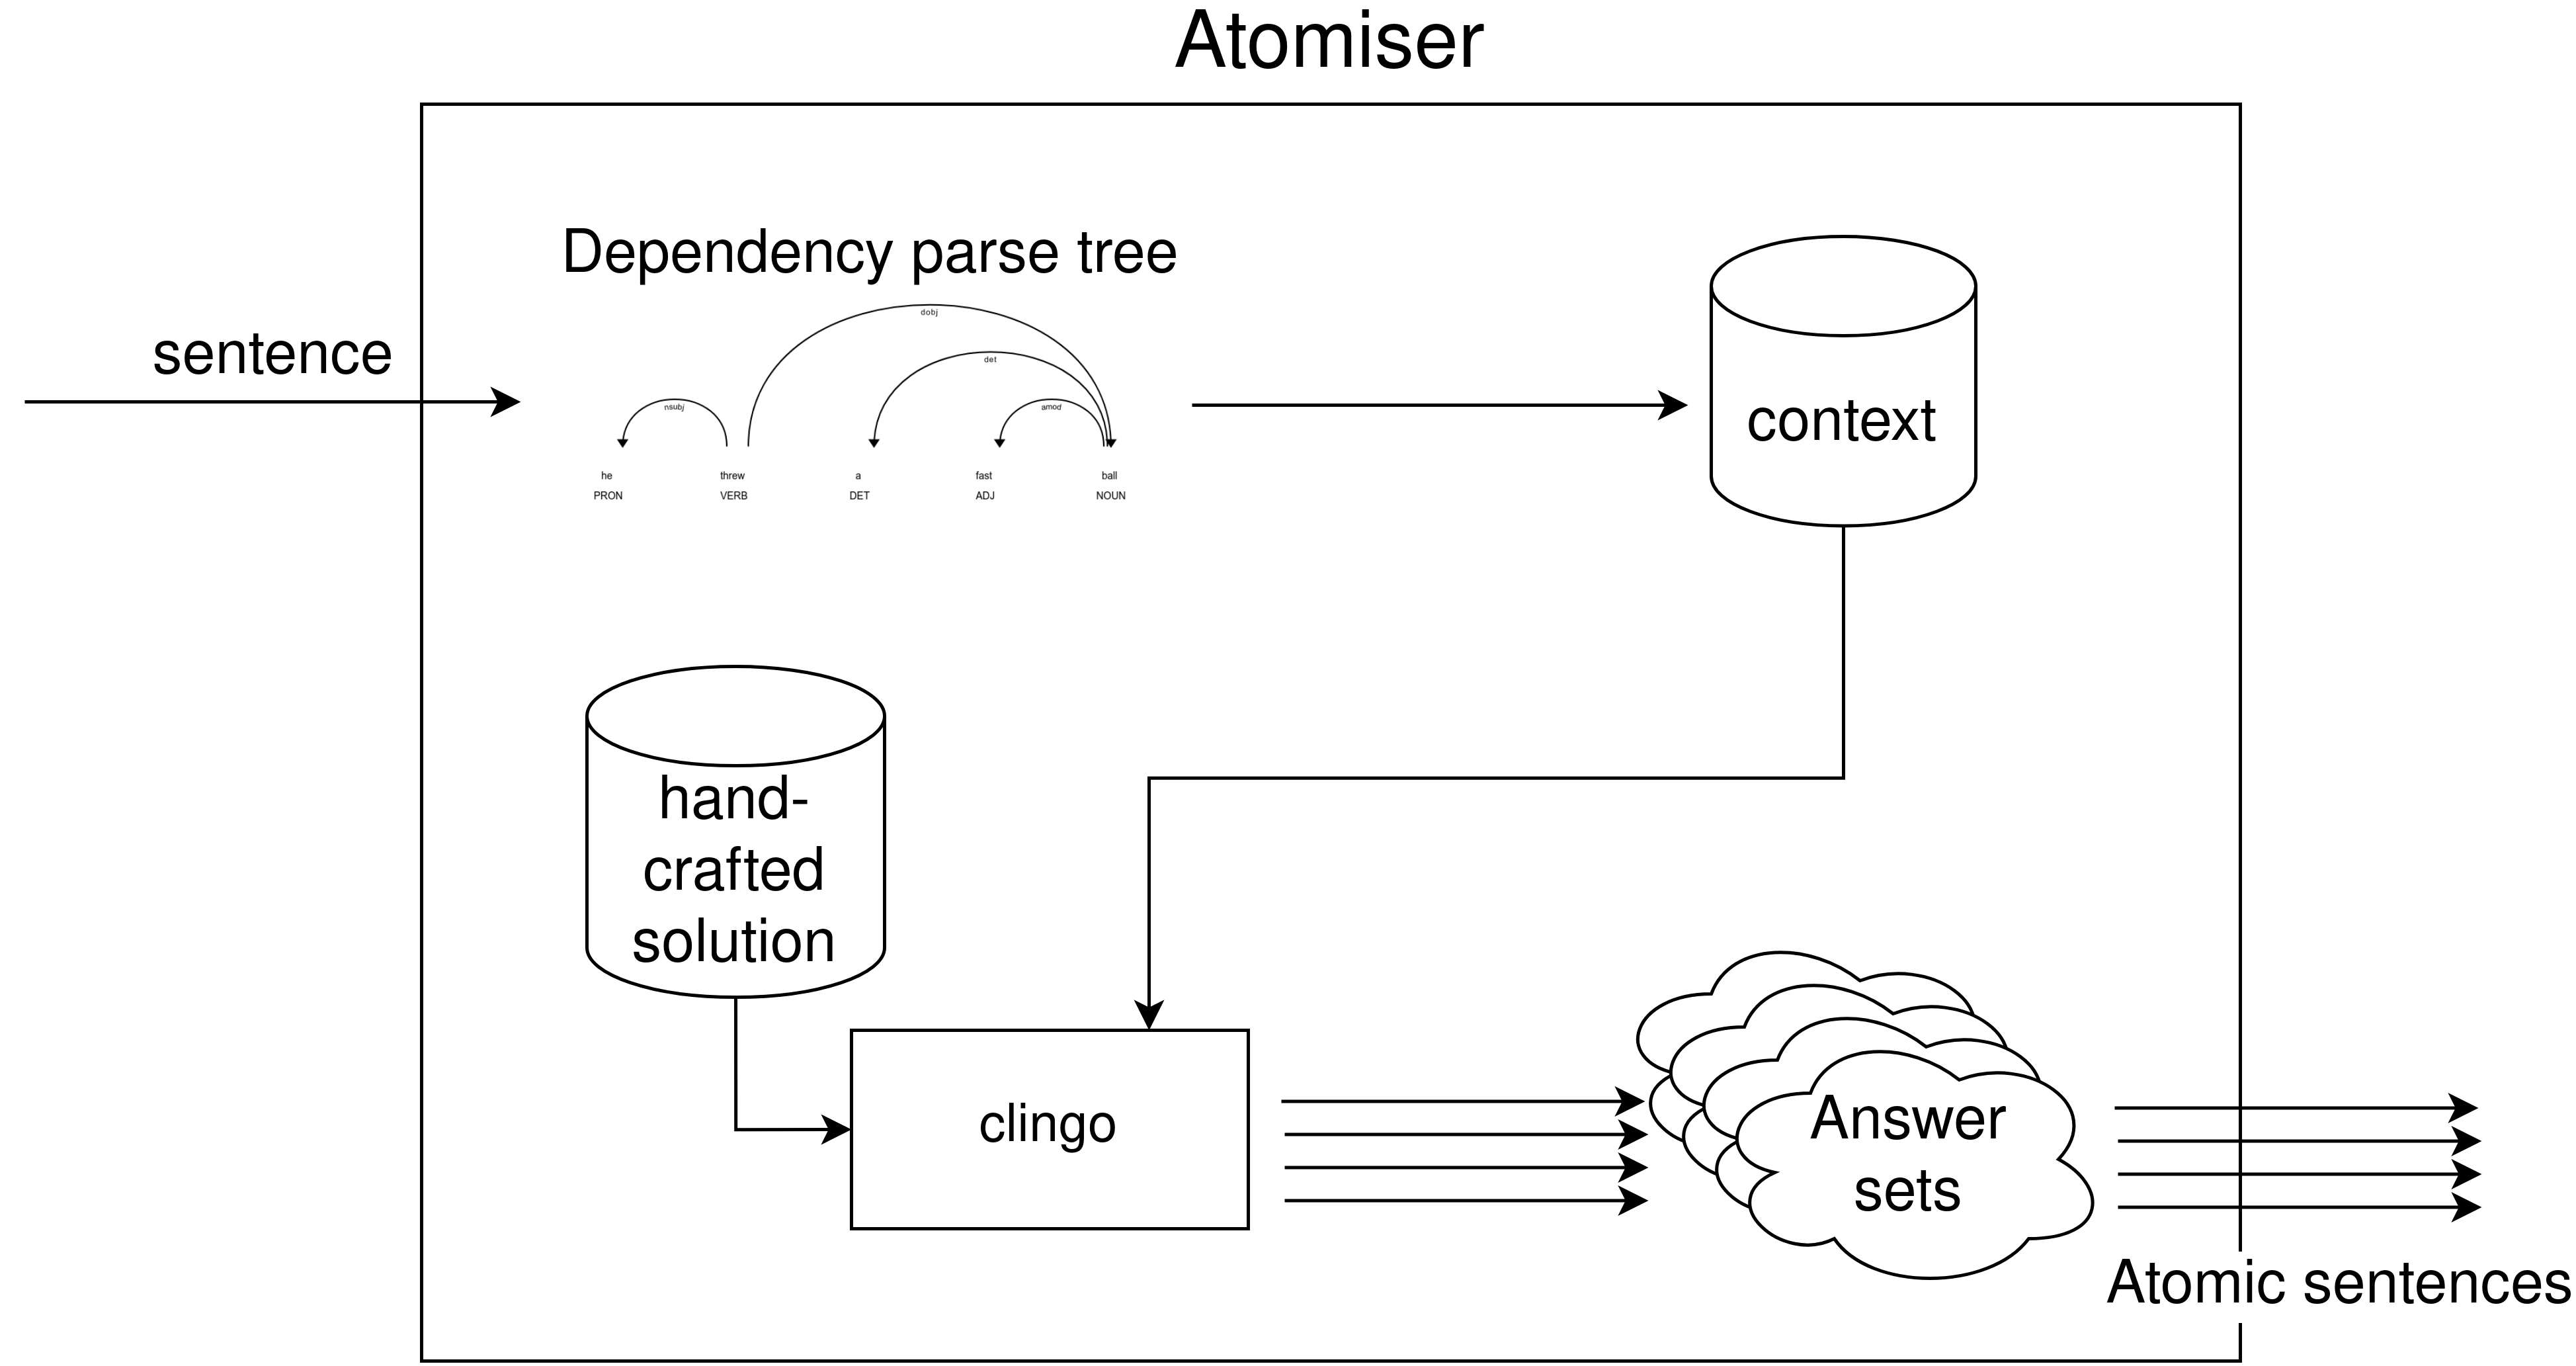
\includegraphics[width=\textwidth]{solving-nlp-tasks-logically/Atomisation diagram.png}
\label{atomisation-diagram}
\end{figure}

In this section, we will introduce the steps the atomiser consists of and demonstrate the idea behind a hand-crafted solution.
% We also showcase that ILASP \cite{RefWorks:RefID:54-ilasp}, a state of the art system for learning answer set programs, is currently not scalable enough to learn a better solution than the hand-crafted one.

\subsection{Logical Encoding of a Sentence}
\label{logical-encoding}

All of the logical encodings presented are compatible with the Answer Set Programming paradigm (\ref{answer-set-programming}), a popular paradigm that deals with negation as failure well.

We first need to define a way to convert a sentence into a logical representation that we could use to reason about the sentence structure.
Ideally, a sentence representation should satisfy the following criteria:
\begin{itemize}
    \item Word dependency capture --- The representation should capture dependencies between words to determine whether a word is crucial to the meaning of a sentence.
    \item Similar meaning $\rightarrow$ similar encoding --- Slight word variations such as words replaced by synonyms should be encoded similarly. The task becomes easier for the learner when the exact representation captures the words with the same meaning.
    \item Compactness --- Smaller representations are quicker to process. 
    \item Domain independence --- We want to apply the generalisation task in various domains, so the representation should not contain domain-specific information.
    \item Interpretability --- It should be clear what the representation encodes. We can translate the learned ILASP solution into English if the predicates are interpretable. Hence, we can verify whether the system learned spurious correlations or valuable rules.
    \item Reconstuctability --- One should be able to reconstruct a sentence as the final output of the task needs to be a correct sentence.
\end{itemize}


% INSERT word2vec reference -Efficient Estimation of Word Representations in Vector Space
A common approach to encoding a sentence involves using dense-vector contextualised embeddings of words, such as the ones produced by word2vec.
Dense-vector embeddings are practical because they are compact and tend to capture the semantics of words (i.e. map similar words to similar value embeddings).
Transformers improve upon these embeddings by using the self-attention mechanism to provide an even better representation of a sentence.

However, dense-vector embeddings are not interpretable, making them difficult to use with our problem. 
The learning approach that we have used follows a similar idea of trying to capture semantic relationships within a sentence.
We utilise the dependency parse tree (\ref{dependency-parsing}) as a basis for the generalisation task as it captures syntactic relationships between words.
Note that the syntactic relationships captured approximate the semantic relationships between words.
In addition, words themselves are put into logical predicates, making the sentences reconstructible.

The dependency tree gives rise to the following predicates:
\begin{verbatim}
    dep(l, token1, token2).
    root(token).
    token(token, string).
\end{verbatim}

It represents that there exists an arc from \verb_token1_ to \verb_token2_ with label \verb+l+ which are converted back to string form with \verb_token_ predicate.
In addition, \verb_root_ encodes which token is the root of the sentence.

\begin{example}
\label{logical-encoding-example}
Encoding \textit{the batter swung and missed}, with a dependency graph shown in \ref{example-dependency-graph}:
\begin{enumerate}
    \item Convert each token in the tree to a logical form
    \begin{verbatim}
        token(tok0, "the").
        token(tok1, "batter").
        token(tok2, "swung").
        token(tok3, "and").
        token(tok4, "missed").
    \end{verbatim}
    \item Convert arcs and roots of the tree to predicates:
    \begin{verbatim}
        root(tok2).
        dep(det, tok1, tok0).
        dep(nsubj, tok2, tok1).
        dep(cc, tok2, tok3).
        dep(conj, tok2, tok4).
    \end{verbatim}
\end{enumerate}
\end{example} 

\begin{figure}[h]
\caption{Dependency graph of \emph{the batter swung and missed}.}
\vspace{10pt}
\centering
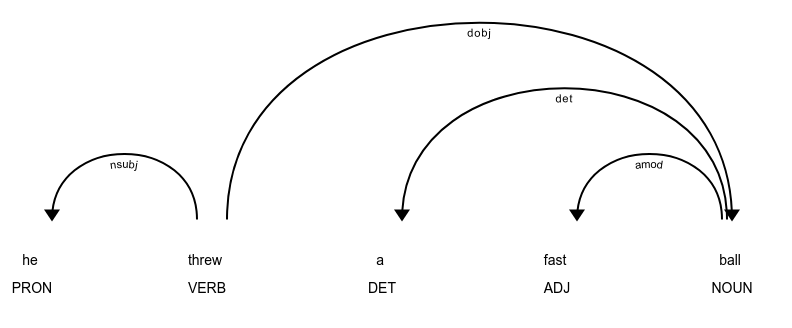
\includegraphics[width=\textwidth]{solving-nlp-tasks-logically/example_dependency_tree.png}
\label{example-dependency-graph}
\end{figure}

Reflecting on the criteria outlined at the start of the section, we can see that it is mainly satisfied by the encoding. 
Even the similar meaning $\rightarrow$ similar encoding is captured somewhat in the context of this problem.
The two sentences which only differ by one synonym would be identically represented by the \verb_dep_ predicates, resulting in any model treating them similarly.
For example, the sentences:
\begin{verbatim}
    The batter hit the ball. The hitter hit the ball.
\end{verbatim}
would have the equal \verb_dep_ predicate representation. 
However, the sentences:
\begin{verbatim}
    The batter hit the ball. The ball was hit by the batter.
\end{verbatim}
would not have similar representations.
This representation drawback was not a hurdle for the current dataset.

\subsubsection{Encoding the Goal}
\label{encoding-the-example-target}

By observing the examples, it became clear that atomic sentences only contained words used in the starting sentence.
We could model the problem in this section as to whether or not we want to include the word in an atomic sentence.
That goal is denoted with a predicate:
\begin{verbatim}
   in_atomic_sent(t).
\end{verbatim}
which represents that a token \verb+t+ is included in the concept sentence.
The possibility of multiple concept sentences existing is modelled using multiple answer sets.
\begin{example}
\label{example-encoding-target}
Encoding \textit{the batter missed} as atomisation of \textit{the batter swung and missed}

From the previous example (\ref{logical-encoding-example}), we have:
\begin{verbatim}
    token(tok0, "the"). token(tok1, "batter"). token(tok2, "swung").
    token(tok3, "and"). token(tok4, "missed").
\end{verbatim}
So, we the example target is encoded as:
\begin{verbatim}
    in_atomic_sent(tok0). in_atomic_sent(tok1).
    in_atomic_sent(tok4).
\end{verbatim}

\end{example}


% TODO: Alessandra feedback: summarise the rules in English first before encoding them symbolically
% TODO: Alessandra feedback: include a table with two columns (predicate name, description) before which highlight what each of the predicates mean (so candidate_start is ...)
\subsection{Hand-crafting the Atomisation Solution}
\label{hand-crafting-the-atomisation-solution}

Consider the following two sentences and the desired atomisation, as well as the dependency graphs of the premises (figure \ref{atomisation-examples}):
\begin{lstlisting}
the batter swung and the ball landed 
  $\rightarrow$ the batter swung. the ball landed.
the batter swung and missed 
  $\rightarrow$ the batter swung. the batter missed.
\end{lstlisting}

\begin{figure}[h]
\caption{Dependency graph of two sentences which need to be atomised}
\centering

\includegraphics[width=\textwidth]{solving-nlp-tasks-logically/dependency-graph-one-subj.png}

\includegraphics[width=\textwidth]{solving-nlp-tasks-logically/dependency-graph-two-subj.png}
\label{atomisation-examples}
\end{figure}

The graph illustrates that the terms on both ends of the \verb_conj_ tag should appear in separate sentences. 
Determining splitting tags, tags whose words should be in distinct subsets, is the core idea of the hand-crafted solution.
The words at the edges of these tags become starting points for generating sentences, which are constructed by adding tokens related to current \verb+in_atomic_sent+ tokens.

The other rules are constructed to add the other necessary sentence tokens.
These may sometimes involve "jumping over" the words at the edge of the splitting tags.
For example, the sentence \verb+The batter swung and missed+ needs to add the associated subject to the \verb_missed_ token to construct a valid sentence.

Following such an approach, the following set of rules was constructed.

\begin{center}
\centering
\begin{tabular}{ |M{5cm}|M{9cm}|  }
 \hline
 \multicolumn{2}{|c|}{Summary of the predicates used} \\
 \hline
 Predicate name & Explanation \\
 \hline
 \hline
 splitting\_tag(Tag) & Tag whose ends should be a part of different sentences \\
 \hline
 candidate\_start(Token) & Token at the edge of a splitting tag \\
 \hline
 in\_atomic\_sent(Token) & Token which should be included in the atomic sentence \\
 \hline
 root(Token) & Root token of a dependency tree \\
 \hline
 dep(Tag, Token, Token) & Arc of a dependency tree \\
 \hline
 adjacent\_subj & Represents whether the current sentence has a subject next to one its tokens \\
 \hline
 do\_not\_include(Tag) & Excludes children arcs with a specific Tag from an atomic sentence. \\
 \hline
\end{tabular}
\end{center}

\begin{lstlisting}

% Capture tokens at the end of a splitting tag
candidate_start(T) :- splitting_tag(C), dep(C, T, _).
candidate_start(T) :- splitting_tag(C), dep(C, _, T).

% Start splitting tags. Splitting tags must be a part of 
% distinct atomic sentences.
1 { in_atomic_sent(T) : candidate_start(T) } 1.

% Root should be a starting point if there are no 
% splitting tags.
in_atomic_sent(T) :- root(T), not candidate_start(_).

% Tags linking tokens that should be in distinct answer 
% sets, each with an example which sparked the choice:

% The batter swung therefore it is a strike.
% $\rightarrow$ The batter swung. It is a strike.
splitting_tag(ccomp).
% The batter did not swing so it was a ball.  
% $\rightarrow$ The batter did not swung. It is a ball.
splitting_tag(advcl).
% The batter swung the bat but missed the ball.
% $\rightarrow$ The batter swung the bat. The batter missed the ball.
splitting_tag(conj).
% The batter hit the ball in play where it was caught 
% mid air by a defender.
% $\rightarrow$ The batter hit the ball in play. It was caught mid air by a defender.
splitting_tag(relcl).



% Include all incoming relationships except candidate_starts. 
% This allows us to reach the predicate of the current atomic sentence.
% Atulve's ball was fast and good.
in_atomic_sent(T) :- dep(_, T, T2), in_atomic_sent(T2), not candidate_start(T).


% Incoming relationships first conjunct (conj) should also be included for the second one.
% This holds for conj only. The clauses tend to be self-sufficient.
% Atulve's ball was good and quick. $\rightarrow$ Atulve's ball was quick. Atulve ball was good.
in_atomic_sent(T) :- dep(_, T, T2), dep(conj, T2, T3), in_atomic_sent(T3), not candidate_start(T).


% Include all children tags apart from those that are blacklisted (we do not want and, therefore...)
% Additionally, we do not want to include a candidate_start token. 

% (Therefore) it is a strike
do_not_include(advmod).
% The batter hit the ball (and) it landed far away.
do_not_include(cc).
% Not including punctuation, it should not be in atomic sentences 
do_not_include(punct).
% The umpire ruled (that) the batter did not swing.
do_not_include(mark).
% Skip all the splitting tags
do_not_include(C) :- splitting_tag(C).
in_atomic_sent(T) :- dep(C, T2, T), in_atomic_sent(T2), not do_not_include(C), not candidate_start(T).

 

% Every atomic sentence should have a subject.
% Include the subject of the first conjunct as a part of the second sentence if it does not contain its own.
% The batter swung but missed the ball $\rightarrow$ The batter swung. The batter missed the ball.
in_atomic_sent(T) :- dep(nsubj, T1, T), dep(C, T1, T2), splitting_tag(C), in_atomic_sent(T2), not adjacent_subj.

% There is no subject next to any currently included token
adjacent_subj :- dep(nsubj, T1, T2), in_atomic_sent(T1).
adjacent_subj :- dep(nsubjpass, T1, T2), in_atomic_sent(T1).
adjacent_subj :- dep(csubj, T1, T2), in_atomic_sent(T1).
adjacent_subj :- dep(csubjpass, T1, T2), in_atomic_sent(T1).
\end{lstlisting}


\subsection{Full pipeline}

The diagram of a whole process, starting from a given sentence to one or many atomic sentences, is shown in the figure \ref{test-architecture-diagram}.

\begin{figure}[h]
\caption{Dependency graph of two sentences which need to be atomised}
\vspace{10pt}
\centering
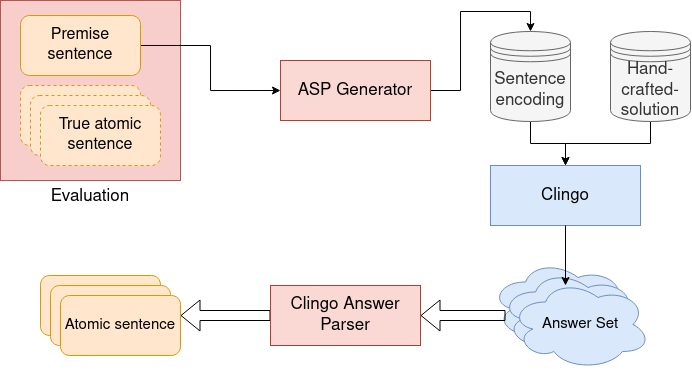
\includegraphics[width=\textwidth]{solving-nlp-tasks-logically/Test architecture diagram.png}
\label{test-architecture-diagram}
\end{figure}

We showcase how it works through an example.

\begin{example}
Generating all of the atomisations of the sentence \emph{The batter swung and missed.} at test time.

The ASPGenerator module carries out the first two steps:

1. Remove . and lowercase all the words in the sentence as a part of pre-processing. The string \emph{the batter swung and missed} is the result of the operations.

2. Convert the sentence to the logical form, as shown by the example \ref{logical-encoding-example}.

The result from step 2 is persisted to the file system as clingo \cite{RefWorks:RefID:22-clingo}, an answer set solver, is a command line tool.

3. The answer set solver is applied with atoms and predicates from the hand-crafted solution (\ref{hand-crafting-the-atomisation-solution}) and the sentence encoding. The resulting clingo output is:
\begin{verbatim}
Answer set #1: 
{in_atomic_sent(tok0), in_generalised_sent(tok1), 
 in_atomic_sent(tok2)}.
    
Answer set #2:
{in_atomic_sent(tok0), in_atomic_sent(tok1), 
 in_atomic_sent(tok4)}.
\end{verbatim}

The Clingo Answer Parser does the last two steps:

4. For each answer set generated, we reconstruct a sentence. 
The sentence reconstruction is done by converting each \verb+in_atomic_sent+ token to the back to its string representation.
They are then joined in the same order they originally appeared.

For instance, the \verb_Answer set #2_ converts the tokens tok0 $\rightarrow$ "the", tok1 $\rightarrow$ "batter", tok4 $\rightarrow$ "missed".
They are joined to a sentence \textit{the batter missed}

5. Post-processing clean-up involving truecasing \ref{nlp-processing-techniques}, which determines the correct word capitalisation, and adding punctuation results in \emph{The batter swung.} and \emph{The batter missed.} \\
\end{example}
 

% TODO: Alessandra feedback: add part 2 of the diagram from the introduction but now show the syntactic parse trees to showcase what we are doing in this part
% TODO: Alessandra feedback: talk about the definition of the learning task associated with the background.
% TODO: Alessandra feedback: make background/language_bias \paragraph or something similar so that they don't appear in the table of contents
\section{Solving Concept Generalisation}
\label{solving-generalisation-task}

The concept generalisation task aims to find a concept sentence from given an atomic sentence.
Recall that a concept sentence is the one obtainable from an atomic sentence through syntactic manipulation which is true if the atomic sentence is.

To tackle this task, we have learned a solution whose application is shown in \ref{generalisation-diagram}.

\begin{figure}[h]
\caption{Diagrammatic representation of the atomiser}
\vspace{5pt}
\centering
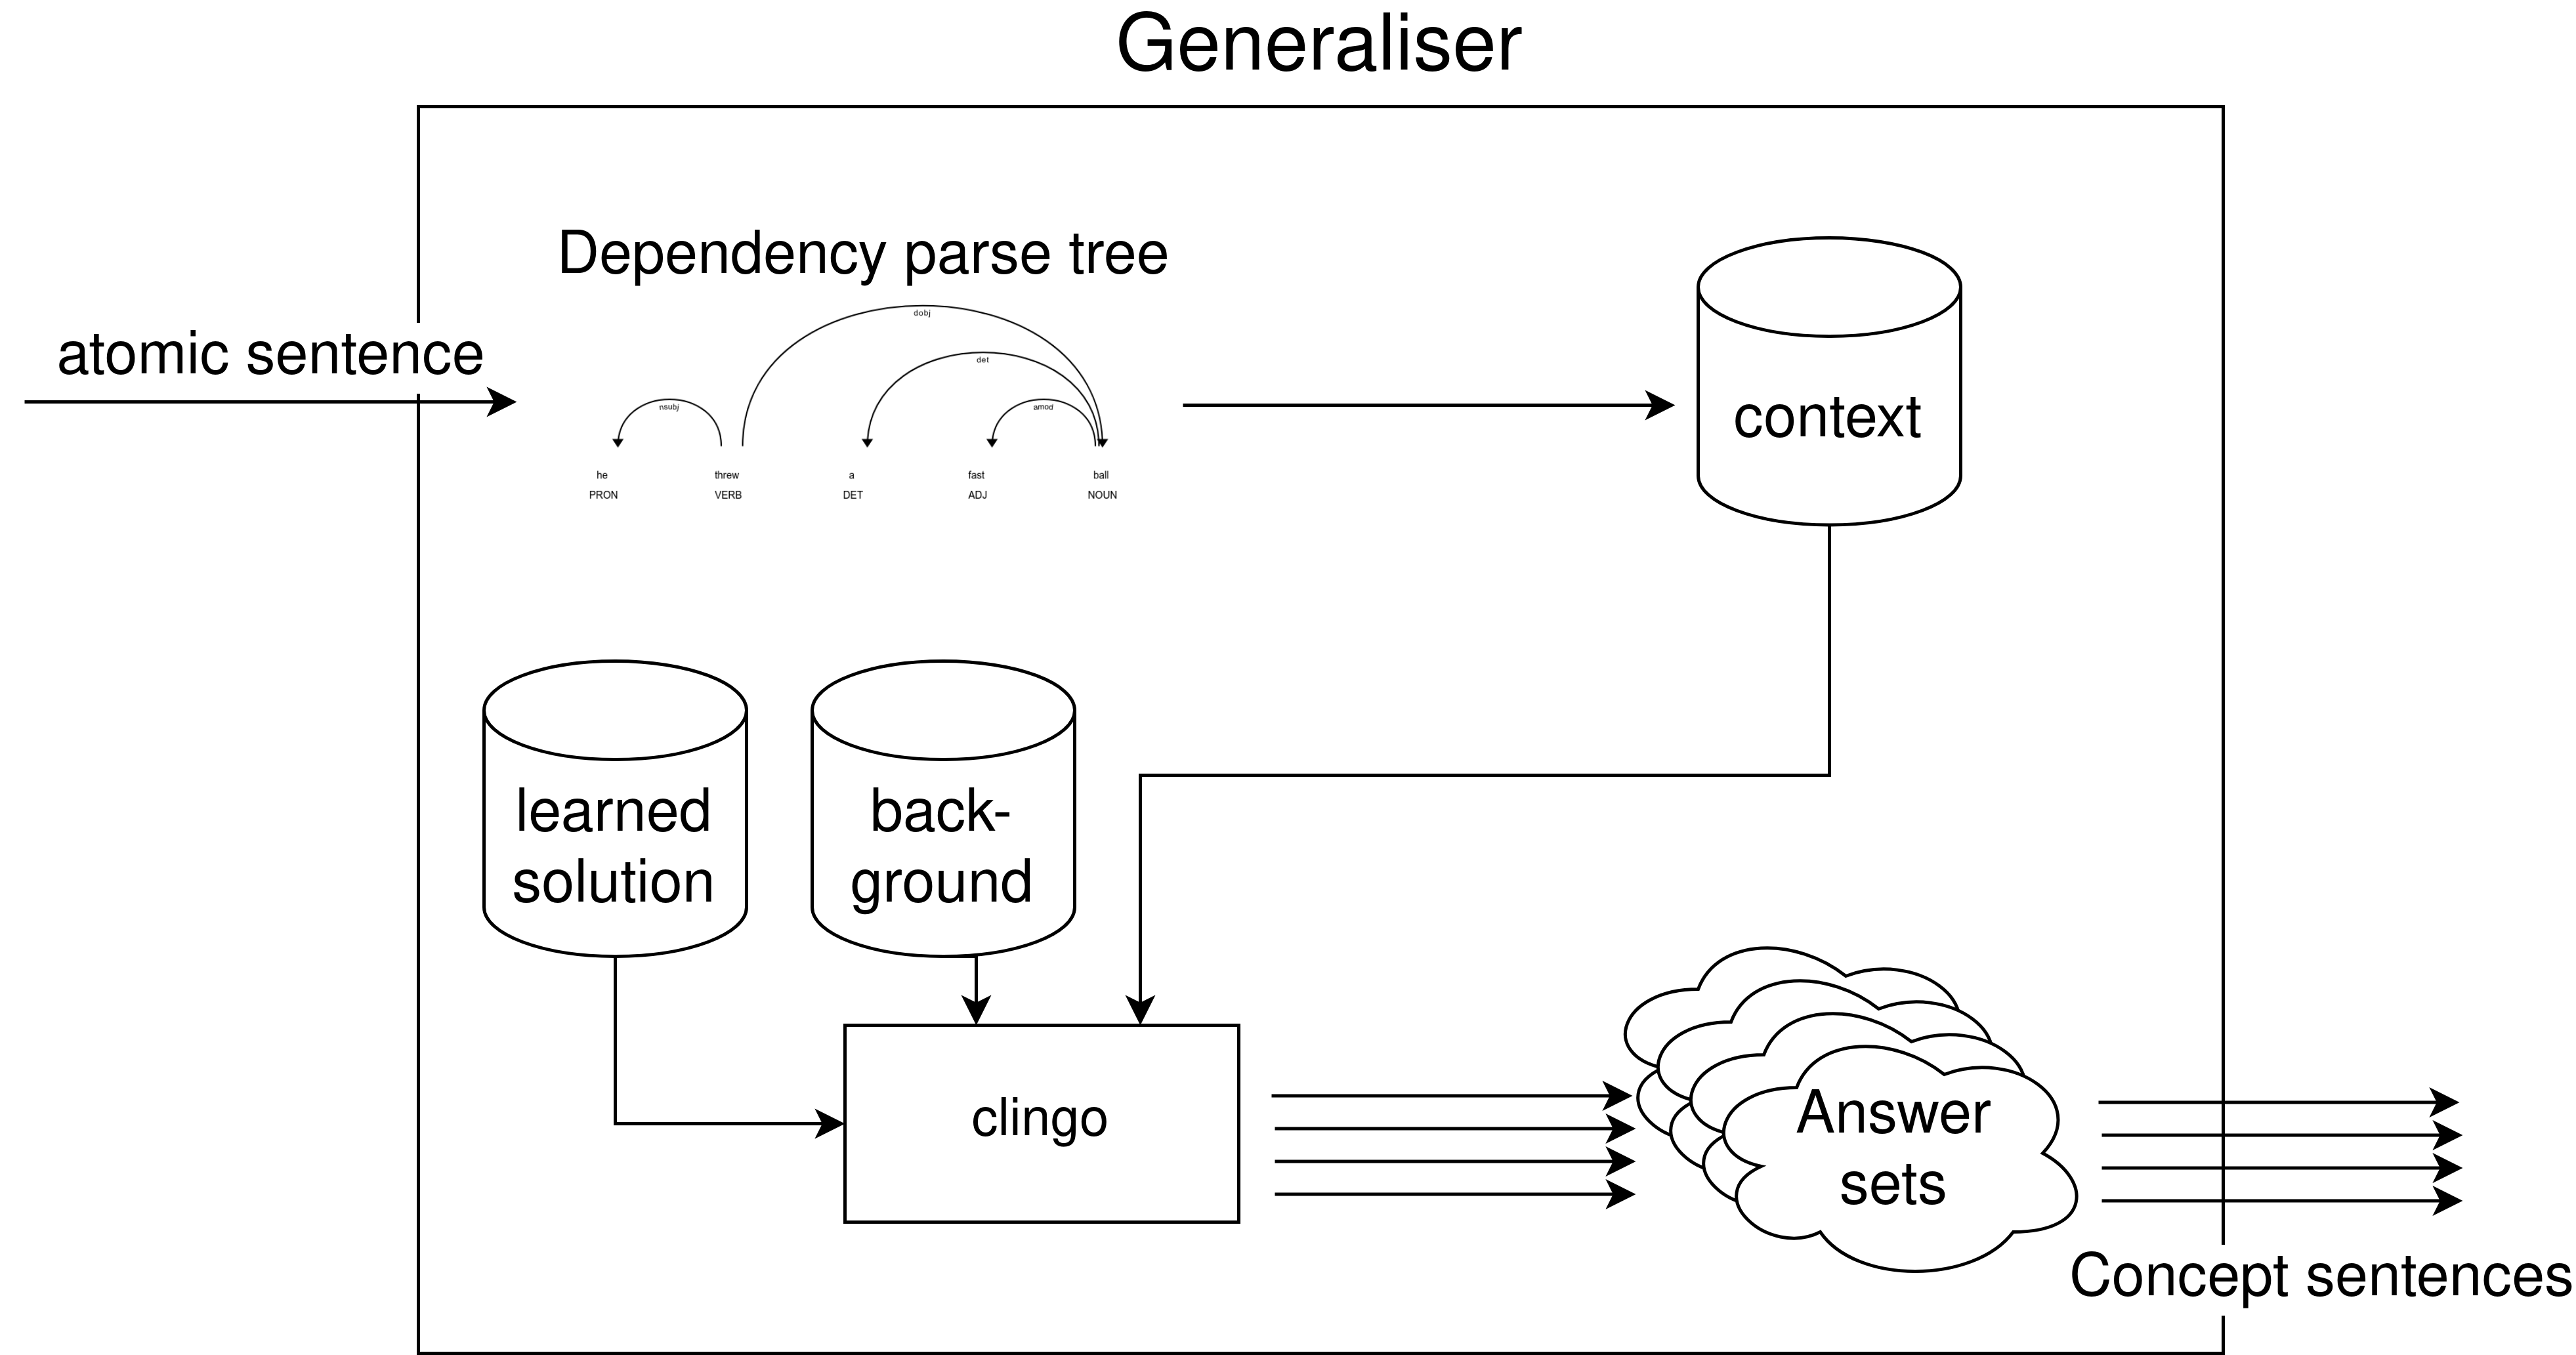
\includegraphics[width=\textwidth]{solving-nlp-tasks-logically/Generalisation Diagram.png}
\label{generalisation-diagram}
\end{figure}

The rule learning is done using ILASP (\ref{ilasp-background}), a state-of-the-art ILP system.

% TODO: fix
\subsection{Encoding the Learning Task}
\label{encoding-the-learning-task}

Learning a solution with ILP is different from determining a solution with Deep Learning.
% INSERT reference to KR notes
Inductive Logic Programming uses a different level of knowledge representation commitment than Deep Learning.
Deep Learning approaches do not give any inductive bias to a machine. 
The model must learn how to solve the problem from the data only. \\
On the other hand, Inductive Logic Programming requires more human-generated knowledge representation.
In particular, the logical structure is encoded to the learner, which is encouraged to find all possible theories within that structure and return the best one. 
Because of this property, the Inductive Logic Programming paradigm can incorporate existing knowledge into the final solution, making the task easier to solve.


\subsubsection{Encoding the Example Premise and Target}

Generalisation examples consist of a given sentence followed by one to many sentences, which are ways in which the provided sentence can be generalised.
For instance, here is a possible generalisation example:
\begin{center}
\setlength\parskip{0pt}
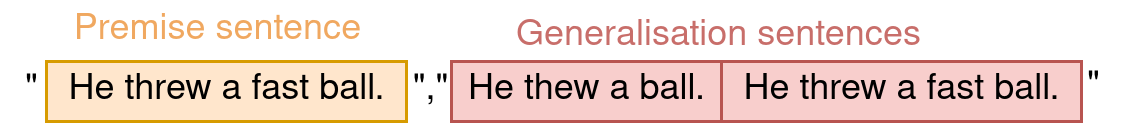
\includegraphics[width=.8\linewidth]{solving-nlp-tasks-logically/raw-generalisation-example.png}
\end{center}

The example premise encoding is equivalent to the procedure for the atomisation task demonstrated in the example \ref{logical-encoding-example}.
Moreover, the example target encoding is also equivalent to the atomisation procedure showcased in the example \ref{example-encoding-target}.
The only difference is that the target is represented by the \verb+in_generalised_sent+ rather than the \verb+in_atomic_sent+ predicate.

% TODO: Alessandra feedback: describe a problem with learner first before going into a hand-crafted solution (after learning)
% Argue that a hand-crafted solution should be something a human engineered ground truth model

\subsubsection{Background Knowledge Construction}

Here is the background knowledge used for the generalisation task.
\begin{verbatim}
token(T) :- root(T).
token(T) :- dep(_, T, _).
token(T) :- dep(_, _, T).
label(L) :- dep(L, _, _).

% there must be a token in any concept sentence
:- #count{T : in_generalised_sent(T)}0.
\end{verbatim}
The first four rules define unary predicates used as types in language bias, while the final rule encodes that a generalised sentence should not be empty.

\subsubsection{Language Bias}

% TODO: Alessandra feedback: Justify a 0 1 boundary
The problem is modelled as a choice of whether a particular token (word) should always be included or sometimes be included in the solution, which the following types of rules can represent.
\begin{verbatim}
in_generalised_sent(T) :- ...
0 {in_generalised_sent(T) } 1 :- ...
\end{verbatim}

This approach gives rise to the following language bias:
\begin{verbatim}
#modeh(in_generalised_sent(var(token))).
#modeha(in_generalised_sent(var(token))).

#modeb(in_generalised_sent(var(token))).
#modeb(root(var(token))).
#modeb(dep(const(label), var(token), var(token)), (positive)).

#bias("
% Only allow rules 0 { in_generalised_sent(V1) } 1.
% Eliminates all generated rules that where lhs of 
% the curly brace is >= 1.
:- in_head(_), lb(1).
").

% Disallow 2+ in_generalised_sent predicates occurring within {}.
#disallow_multiple_head_variables.

\end{verbatim}

% TODO: Alessandra feedback: what would happen if we only had #pos examples.
% TODO: Alessandra feedback: Argue that the size is because of the number of constants that we have. 
\subsubsection{Example Encoding}
\label{example-encoding}

As mentioned, generalisation examples consist of a given atomic sentence followed by 1 to many concept sentences.
We need to convert those representations into ILASP examples.
ILASP allows defining two types of examples as outlined in \ref{examples-in-ilasp}.
\begin{itemize}
    \item positive (\verb_#pos_) - an example which should be by at least one answer set.
    \item negative (\verb_#neg_) - an example that any answer set should not extend.
\end{itemize}

Ideally, we want the solution learned by ILASP to produce the number of answer sets equal to the number of generalisations.
Using these two constructs, we can define that we want precisely one answer set for each possible generalisation. \\
It is done by creating a positive example for each sentence we wish to produce. 
In addition, a negative example is produced with the \verb_goal_ predicate in the exclusion for each text sentence example.
The \verb_goal_ predicate, defined only in the contexts of negative examples, is true if \verb+in_generalised_sent+ atoms correspond precisely to a positive example.


\begin{example}
Generating ILASP-compatible generalisation examples for \textit{"He threw a fast ball.", "He threw a ball. He threw a fast ball."}

% INSERT reference to previous section %
1. Convert the premise sentence to logical form (analogous to \ref{logical-encoding-example}), resulting in tokens:
\begin{verbatim}
    token(tok0, "he"). token(tok1, "threw").
    token(tok2, "a"). token(tok3, "fast").
    token(tok4, "ball"). root(tok1).
    dep(nsubj, tok1, tok0). dep(dobj, tok1, tok4).
    dep(det, tok4, tok2). dep(amod, tok4, tok3).
\end{verbatim}

as shown in the example \ref{logical-encoding-example}.

2. For each possible generalisation, create a positive example. The context consists of predicates produced in step 1, while the inclusion/exclusion of appropriate \verb+in_generalised_sent+ tokens (analogous to \ref{example-encoding-target}). The concept sentence \textit{He threw a ball.} yields the following example:
\begin{verbatim}
#pos(example_id@noise_penalty,
{in_generalised_sent(tok0), in_generalised_sent(tok1), 
 in_generalised_sent(tok2), in_generalised_sent(tok4), 
 in_generalised_sent(tok5)},
{in_generalised_sent(tok3)}, % tok3 = "fast"
{
% all the predicates generated in step 1
}).
\end{verbatim}
We would also construct a similar example for \textit{He threw a fast ball}.

3. The negative example is generated as follows:
\begin{verbatim}
#neg(example_id@noise_penalty,
{ },
{ goal },
{
% all the predicates generated in 1)

% He threw a fast ball.
goal :- in_generalised_sent(tok0), in_generalised_sent(tok1), 
        in_generalised_sent(tok2), in_generalised_sent(tok3), 
        in_generalised_sent(tok4), in_generalised_sent(tok5).
% He threw a ball.
goal :- in_generalised_sent(tok0), in_generalised_sent(tok1), 
        in_generalised_sent(tok2), in_generalised_sent(tok4), 
        in_generalised_sent(tok5)}, not in_generalised_sent(tok3).
}).
\end{verbatim}
\end{example}

All the examples constructed have a \verb+noise_penalty=1+ as the concept generalisation examples may be noisy.

\subsection{Final Solution}

ILASP is not nearly scalable enough to solve the task presented in this section. Still, with the optimisations from the next section, it can return a high-performing solution.
In addition, we ran all ILASP tasks with the \verb+--restarts+ flag, which can help reduce the running time of a program.

The generalisation task performance is evaluated in \ref{concept-generalisation-results}.

% TODO: Alessandra feedback: scaling up should be a separate section
\section{Managing Learning Scalability Constraints}

% INSERT reference for this. %
A considerable challenge with logic-based learning systems, such as ILASP, is a lack of scalability when dealing with large-scale AI problems compared to other forms of machine learning. \\
For the generalisation task, two challenges needed to be mitigated: 
\begin{itemize}
    \item Lack of scalability w.r.t size of the hypothesis space -- This issue arises due to ILASP enumerating search space $S_M$ in full before finding a solution.
    \item Extreme RAM consumption during task solving.
\end{itemize}

\subsubsection{Reducing the hypothesis space size}
\label{reducing-the-hypothesis-space-size}

Since ILASP is not particularly scalable w.r.t to the size of the hypothesis space, the only option left was to reduce it.

For example, consider the following simplified language bias definition:
\begin{verbatim}
#modeh(in_generalised_sent(var(token))).
#modeb(in_generalised_sent(var(token))).
#modeb(root(var(token))).
#modeb(dep(const(label), var(token), var(token))).

... all the constant definitions ...
\end{verbatim}

% INSERT Might be benficial to include a table how each rule reduced the search space size.

It took over 13 hours to generate an entire search space on a machine with an Intel Core i7 10510U 1.80GHz / 4.90GHz processor and 16 GiB of RAM.

FastLAS \cite{RefWorks:RefID:19-law2020fastlas:} is a system designed to alleviate this particular constraint, but it can only deal with a restricted version of the learning task.
Its inability to deal with recursion made it inapplicable for the current problem.

% INSERT reference to Mark's website https://doc.ilasp.com/specification/meta_asp_hypothesis_space.html
The scalability issue was tackled using meta-level definitions of the hypothesis space, which allow much greater flexibility than simple \textit{modeb}, \textit{modeh} statements. 
They allow constraining how rules are generated using ASP syntax, removing rules that we do not want as a part of the learned solution.
We always want to remove the rules whose body could never be satisfied.

Here are some examples of how they are utilised to restrict the generalisation search space:
\begin{verbatim}
% Idea #1: Dep represents an arc in a tree. This allows 
% cutting out rules which are impossible to be satisfied.
    
% It is impossible to have more than 1 root per example.
:- #count{T : body(root(T))} > 1.

% Trees cannot have a relation to itself.
:- body(dep(_, X, X)).
:- body(naf(dep(_, X, X))).

% A tree is not symmetric.
:- body(dep(_, X, Y)), body(dep(_, Y, X)).

% No dependency can go to the root
:- body(root(X)), body(dep(_, _, X)).

% Idea #2: Only allow two dep rules to occur in a body
% under certain conditions. 

% Pairs of dependency tags which can co-occur.
% Much smaller set of all possible pairs.
dep_chain(prep, pobj).
dep_chain(pobj, amod).
...

% Allow any rule with at most one dep predicate
allowed_dep_rule :- #count{L, V4, V5 : body(dep(L, V4, V5))} <= 1.
% Allow rule with two dep predicates if it is labels are white-listed
% by dep_chains and tokens are chained too.
allowed_dep_rule :- body(dep(L1, _, V2)), body(dep(L2, V2, _)), 
                    dep_chain(L1, L2), 
                    #count{L, V4, V5 : body(dep(L, V4, V5))} = 2.

:- not allowed_dep_rule.

% Idea 3: Remove rules that where simpler rules would suffice.

% Rule with root(V3) where V3 is not used in any dep is not needed.
% This predicate is trivially satisfied since every sentence has a 
% root.
:- body(root(X)), not body(dep(_, X, _)), not body(dep(_, _, X)), 
   body(dep(_, _, _)).

% If we have a in_generalised_sent predicate there must be some logic 
% related to it.
% This predicate is trivially satisfied otherwise, since the 
% background requires that at least one must always exist.
:- body(in_generalised_sent(X)), not body(dep(_, X, _)), 
   not body(dep(_, _, X)).


\end{verbatim}

These modifications allowed the search space generation times to take less than a minute, starting from over 13 hours.
The final search space consisted of only 3652 rules.


% TODO: Alessandra feedback: avoid using OOM acrynoym - replace with out-of-memory/lack of memory
\subsubsection{Avoiding OOM Errors}
\label{avoiding-oom-errors}

\begin{figure}[h]
\caption{Comparison of the ILASP solution performance and memory consumption over time. A lower ILASP score corresponds to a better solution.}
\centering
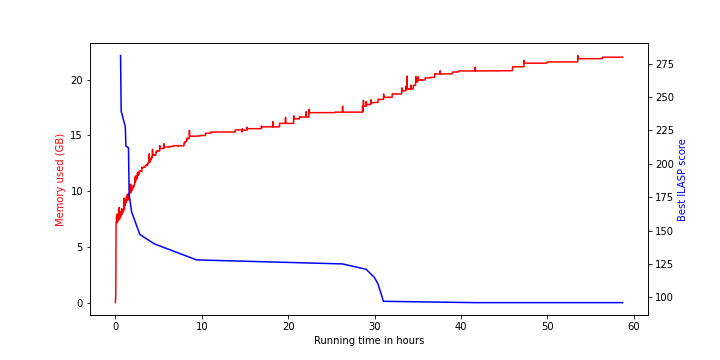
\includegraphics[width=\textwidth]{solving-nlp-tasks-logically/generalisation_memory_vs_best_score.png}
\label{generalisation-memory-graph}
\end{figure}

ILASP memory consumption is drastic even for the simpler of the two tasks solved logically.
% INSERT memory graph drawn on batch machine over time for generalisation.
The memory consumption graph over time is outlined in \ref{generalisation-memory-graph}.
As seen in the plot, the graph is around 15 GB of RAM at about the 15-hour mark.
So, to prevent the usual 16 GB machines from going out of memory, the execution is terminated after 15 hours, and the best solution found until that point is returned.
This technique prevents the ILASP process from exceeding the memory limit while returning a high-quality result.

% INSERT reference to PyLASP doc https://ilasp.com/PyLASP
The aforementioned ILASP behaviour modification is possible through the use of PyLASP scripts.

\subsection{Atomisation Learning Challenges}
\label{atomisation-learning-challenges}

Recall that the atomisation is only solved using the hand-crafted solution. 
In this section, we highlight why it is not currently possible to learn a good atomisation solution with ILASP.

We aimed to learn two things with ILASP for the atomisation learning task:
\begin{enumerate}
    \item A set of rules which extend the number of tokens in the current atomic sentence.
    \item A set of splitting tags.
\end{enumerate}

Constructing the language bias by observing the hand-crafted solution gives results in the following code:
\begin{verbatim}
#modeh(in_atomic_sent(var(token))).
#modeh(splitting_tag(const(label))).

#modeb(1, dep(const(label), var(token), var(token)), (positive)).
#modeb(1, dep(var(label), var(token), var(token)), (positive)).
#modeb(1, splitting_tag(var(label))).
#modeb(1, in_atomic_sent(var(token)), (positive)).
#modeb(1, do_not_include(var(label))).
#modeb(1, candidate_start(var(token))). 
#modeb(1, adjacent_subj).

% Add only negative atoms
#bias("
:- body(adjacent_subj).
:- body(candidate_start(_)).
:- body(do_not_include(_)).
").
\end{verbatim}

The language bias additionally included a more aggressive alternative to the search space reduction method presented in \ref{reducing-the-hypothesis-space-size}, but had all of the rules the hand-crafted solution uses. \\
In addition, we constructed the examples in the same manner as in \ref{example-encoding}.
The learning was done on a specialised machine with 500 GiB of RAM, but it still required that an approximate solution be returned after some time (\ref{avoiding-oom-errors}).

% TODO: Alessandra feedback: replace prior with size in the graph legend
% TODO: Alessandra feedback: suggest that ... is the lower bound to solve the task. In addition suggest that if that lower bound was achieved the performance would be at least as good as the ... blue line
% TODO: Alessandra feedback: suggest that the green line is the maximum size the ILASP hypothesis can have
% TODO: Alessandra feedback: talk about ILASP score in background, reference in graph

\begin{figure}[h]
\caption{Comparison of the ILASP atomisation solution performance and memory consumption over time. The dashed lines represent the values the hand-crafted solution would achieve had it been learned by ILASP.} 
\centering
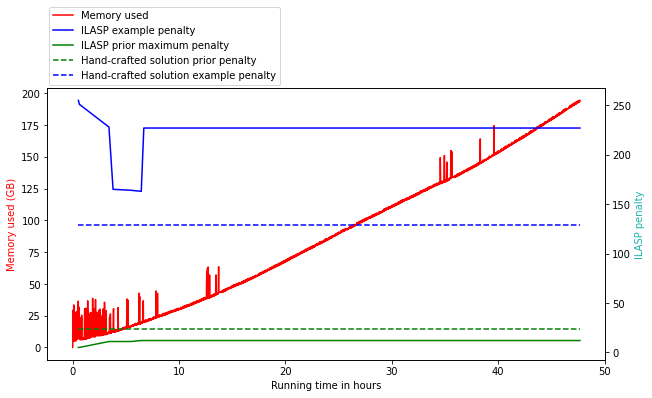
\includegraphics[width=\textwidth]{solving-nlp-tasks-logically/atomisation_memory_vs_best_score.png}
\label{atomisation-memory-graph}
\end{figure}

% INSERT reference Mark thesis Inductive learning of answer set programs % 
ILASP can theoretically find the optimal solution for any noisy task, and the search space represents the hand-crafted solution in full. 
So, we expect the complete run of the task to produce at least as good of a solution as the hand-crafted one.
However, as shown in \ref{atomisation-memory-graph}, this expectation does not hold within the memory and time constraints available for the \textbf{atomisation} task.

Recall that in a noisy setting, the score ILASP minimises is the sum of the hypothesis length and uncovered example penalties.
The hand-crafted solution would have had the score of 24 (hypothesis length) + 129 (uncovered example penalty) = 153.
However, the graph \ref{atomisation-memory-graph} showcases that the learned solution never reaches those values.
The maximum hypothesis length the ILASP allowed never went above 12. 
Had the learner raised the hypothesis length limit to at least 24, it could have found a solution with a smaller or equal noise penalty to the hand-crafted one.

The learner is unlikely to attempt as complex of a solution before the memory runs out. 
The memory consumption is quickly increasing while the maximum hypothesis score is staying flat in the graph \ref{atomisation-memory-graph}.
This behaviour may even suggest a presence of a bug.

\section{Evaluation}

\subsection{Metrics}


% TODO: Alessandra feedback: talk about metrics such as Jaccard@5, Jaccard@0.1 where the former allows Levensthein distance to be <= 5 for the result to be correct and the latter allows Edit distance to be <= 0.1 length

Both atomisation and generalisation problems had a set of solutions of unknown size.
A needed metric would give a higher score if two sets are very similar compared to those far apart.

There were three metrics which we measured for that reason: Jaccard Index, Set-Recall, and Set-Precision:

$Jaccard \; Index$ is a metric defined as follows:
\begin{itemize}
   \item $Jaccard(A, B) = \frac{card(A \cap B)}{card(A \cup B)}$, where $card$ represents set cardinatlity, $A$ a set containing the true solutions, while $B$ contains the predicated solutions.\\
\end{itemize}
It measures the overlap between the two sets.
 
$Set-Precision$ and $Set-Recall$ are defined in the similar manner as the $Precision$ and $Recall$ in the classification context:
\begin{itemize}
    \item $Set-Precision(A, B) = \frac{card(A \cap B)}{card(B)} = \frac{number \; of \; correctly \; predicted \; sentences}{number \; of \; predicated \; sentences}$
    \item $Set-Recall(A, B) = \frac{card(A \cap B)}{card(A)} = \frac{number \; of \; correctly \; predicted \; sentences}{number \; of \; correct \; sentences} $ 
\end{itemize}
where $card$ represents set cardinality, $A$ a set containing true solutions, while $B$ contains predicated solutions. 
These two metrics help better understand the type of errors the model makes.


% Contains more sophisticated metrics if needed.
% That would ideally involve a similarity in number of produced solutions and similarity of the elements themselves.
% 
% Due to this reason, a single number would have been hard to interpret since it would make it unclear what kinds of mistakes the model is making. 
% For that reason, the evaluation is done with metrics which work with sets with possibly reduced notion of element equality.
% 
% 
% These metrics are also evaluated in a slightly relaxed manner using Levensthein distance.
% $Jaccard\text{-}k$ is a notation used in this report where two elements of a set are equal if their Levensthein distance is less or equal $k$.
% The same notational trick is used for $Recall\text{-}k$ and $Precision\text{-}k$.
% 

% TODO: Alessandra feedback: Show a learned H because it is interpretable (might want to do some analysis there)
\subsection{Concept Generalisation}
\label{concept-generalisation-results}

\subsubsection{Cross-validation results}

Due to only 130 examples available, we are using 10-fold cross validation to get the results for this chapter.
In addition, to complete the execution with 16 GB of RAM, the computation is cut after 12 hours of running time (as argued in \ref{avoiding-oom-errors}).

The results are summarised in the table below:

\begin{center}
\centering
\begin{tabular}{ |M{3cm}||M{3cm}|M{3cm}|M{3cm}|  }
 \hline
 \multicolumn{4}{|c|}{Summary of results} \\
 \hline
  &Jaccard Index&Precision&Recall\\ 
 \hline
 Training  & 0.92 $\pm$ 0.00 & 0.95 $\pm$ 0.00 & 0.95 $\pm$ 0.00 \\
 Test & 0.85 $\pm$ 0.03 & 0.89 $\pm$ 0.02 & 0.89 $\pm$ 0.02 \\
 \hline
\end{tabular}
\end{center}

Overall, the results are relatively high, with >85\% test Jaccard Index value.
This result means that given a set of true sentences and a set of predicted sentences, more than 85\% will match exactly.
Looking into more detail the types of mistakes the final model makes, they can be subdivided into three groups:

% INSERT how often each occurs for one solution % 
\begin{itemize}
    \item Genuine errors --- The learned solution fails to produce the examples correctly.
    \item Borderline errors --- The solution does not precisely match the provided gold standard. However, the produced solution might have been made by another data annotator. So, it is probably sufficiently good.
    % INSERT reference: https://spacy.io/models/en#en_core_web_lg
    \item Parser errors --- The dependency parser is imperfect, which can be seen as the cause of some incorrect solutions. For example, a more accurate transformer parser labels \textit{foul ball} as a compound of nouns, whereas the CPU-optimised one used in the project believes \textit{foul ball} has an adjective. The reported LAS accuracy of the CPU-optimised parser is 0.9.
\end{itemize}

Finally, in all experiments, $Set$-$Precision$ and $Set$-$Recall$ were similar, meaning that missing a solution and producing an incorrect one were similarly likely.


\subsubsection{Comparison with the Manually-Engineered Solution}

The hypothesis was learned and engineered on a subset of the MLB-V2E dataset \cite{RefWorks:RefID:16-2021automatic}.
% INSERT CUB reference
We compare their performance on the MLB-V2E dataset and a subset of the CUB-bird dataset \cite{RefWorks:RefID:69-wah2011caltech-ucsd}, an out-of-domain dataset.
The former dataset consists of 120 generalisation examples, while the latter has 100 samples.

The results are summarised in tables below:

\begin{center}
\begin{tabular}{ |M{3cm}||M{3cm}|M{3cm}|M{3cm}|  }
 \hline
 \multicolumn{4}{|c|}{In Domain Dataset} \\
 \hline
 \hline
  &Jaccard Index&Precision&Recall\\ 
 \hline
 Hand-crafted $H$ & 0.79 $\pm$ 0.03 & 0.86 $\pm$ 0.03 & 0.80 $\pm$ 0.03 \\ 
 Learned $H$ & 0.92 $\pm$ 0.02 & 0.95 $\pm$ 0.02 & 0.94 $\pm$ 0.02 \\
 \hline
\end{tabular}
\end{center}

\begin{center}
\begin{tabular}{ |M{3cm}||M{3cm}|M{3cm}|M{3cm}|  }
 \hline
 \multicolumn{4}{|c|}{Out Of Domain Dataset} \\
 \hline
 \hline
  &Jaccard Index&Precision&Recall\\ 
 \hline
 Hand-crafted $H$ & 0.71 $\pm$ 0.04 & 0.72 $\pm$ 0.03 & 0.83 $\pm$ 0.04 \\ 
 Learned $H$ & 0.83 $\pm$ 0.03 & 0.84 $\pm$ 0.03 & 0.86 $\pm$ 0.03 \\ 
 \hline
\end{tabular}
\end{center}

As expected, the performance is higher with the in-domain dataset.
The out-of-domain dataset evaluation leads to a ~10\% Jaccard Index reduction for both methods. 
The drop is a result of the distribution shift between the two datasets.
In particular, one of the main reasons for the drop in performance is the lack of accounting for the \verb_acomp_ tag (e.g. tag between \textit{is} and \textit{red} in \textit{A bird is red}).
It barely occurs in the MLB-V2E dataset, so both solutions fail to account for it.



\subsection{Atomisation}

There is no cross-validation evaluation of the ILASP output due to a poorly learned solution and high computation requirements (\ref{atomisation-learning-challenges}).
However, the best-learned solution is still compared to the hand-crafted one to showcase how far it is from the manually generated one.
To better showcase the poor performance of the learned solution, simple $H$, a hypothesis which always returns the sentence in full, is introduced.

\subsubsection{Comparison of the Learned and Manually Generated Solutions}

The results averages and standard errors are presented in the tables below:

\begin{center}
\begin{tabular}{ |M{3cm}||M{3cm}|M{3cm}|M{3cm}|  }
 \hline
 \multicolumn{4}{|c|}{In Domain Dataset} \\
 \hline
 \hline
  &Jaccard Index&Set-Precision&Set-Recall\\ 
 \hline
 Simple $H$ & 0.18 $\pm$ 0.04 & 0.18 $\pm$ 0.04 & 0.18 $\pm$ 0.04 \\ 
 Hand-crafted $H$ & 0.55 $\pm$ 0.04 & 0.61 $\pm$ 0.04 & 0.63 $\pm$ 0.04 \\ 
 Learned $H$ & 0.38 $\pm$ 0.04 & 0.42 $\pm$ 0.04 & 0.43 $\pm$ 0.04 \\ 
 \hline
\end{tabular}
\end{center}

% TODO: Alessandra feedback: Ale suggested the name empty H, but it may not be completely correct.
% TODO: Alessandra feedback: Discuss number more, what does 0.09 mean essentially
% TODO: Alessandra feedback: Include snippet of the data that have certain characteristics, for example when elaborating on what doesn't work 

\begin{center}
\begin{tabular}{ |M{3cm}||M{3cm}|M{3cm}|M{3cm}|  }
 \hline
 \multicolumn{4}{|c|}{Out Of Domain Dataset} \\
 \hline
 \hline
  &Jaccard Index&Set-Precision&Set-Recall\\ 
 \hline
 Simple $H$ & 0.06 $\pm$ 0.02 & 0.06 $\pm$ 0.02 & 0.06 $\pm$ 0.02 \\ 
 Hand-crafted $H$ & 0.51 $\pm$ 0.04 & 0.55 $\pm$ 0.04 & 0.57 $\pm$ 0.04 \\ 
 Learned $H$ & 0.09 $\pm$ 0.02 & 0.11 $\pm$ 0.03 & 0.11 $\pm$ 0.03 \\ 
 \hline
\end{tabular}
\end{center}

The hand-crafted solution vastly outperforms the learned one, with a 45\% Jaccard Index improvement.
Nevertheless, even the hand-crafted solution has room for improvement as the Jaccard Index value is at 0.55.
This result means that given a set of true sentences and a set of predicted sentences, we expect that 55\% will match exactly.
The Jaccard Index value, however, is the worst-case estimate.
In some cases, the output is well enough even though it is not exactly correct.
For instance, consider the sentence:
\begin{lstlisting}
The pitcher threw the ball which was high. 
  $\rightarrow$ The pitcher threw the ball. The ball was high.
\end{lstlisting}
This sentence is spilt with the current model into \verb+The pitcher threw the ball.+ \verb+Which was high.+, resulting in the Jaccard Index value of 0.333.

Nevertheless, the sentence \verb+Which was high+ is often sufficiently good for downstream tasks.
For example, it would be grouped with a valid sentence \verb+It was high+ in our concept bottleneck pipeline (Chapter \ref{concept-bottleneck-pipeline}). \\
Also, the presented sentence contains a relative clause, which was a significant hurdle for the hand-crafted solution.
It requires that the ends of the splitting tag be in the same atomic sentence, which clashes with the existing core atomisation idea (\ref{hand-crafting-the-atomisation-solution}).


The out-of-domain dataset results in a 0.04 Jaccard Index drop for the hand-crafted hypothesis.
However, that dataset seems better suited for the \verb+splitting_tag+ logic used since the sentences presented were less grammatically complex.
The sentences mainly contained conjunctions with sub-clauses rarely appearing.
The poor result comes from splitting the sentences with multiple conjuncts, which were unaccounted for in the hand-crafted solution.

On the other hand, the learned solution performs terribly on the out-of-domain dataset.
There is no conclusive evidence that it consistently outperforms the simple hypothesis, as there is an overlap between the respective $Jaccard$-$Index$ values.

Finally, in all experiments, $Set$-$Precision$ and $Set$-$Recall$ values were similar, meaning that missing a solution and producing an incorrect one was similarly likely.

